%%%%%%%%%%%%%%%%%%%%%%%%%%%%%%%%%%%%%%%%%%%%%%%%%%%%%%%%%%%%%%%%%%%%%%%%%%%
% Assignment 6.2: Performing an ANOVA in R
%%%%%%%%%%%%%%%%%%%%%%%%%%%%%%%%%%%%%%%%%%%%%%%%%%%%%%%%%%%%%%%%%%%%%%%%%%%

\rassignment{Assignment 6.2: Performing an ANOVA in R}

Now let’s extend the analysis from assignment 6.1 by comparing all four groups (\rcode{Blue}, \rcode{Brown}, \rcode{Green}, \rcode{Down}) instead of only the \rcode{Blue} and \rcode{Brown} groups. When you are testing more than two \concept{means}, you can use an \concept{ANOVA} test (a specific form of regression). Since you want to compare all four groups, you can leave the \rcode{ttestData} from the previous assignment and focus on the data in \rcode{dataset8}. Remember that you are interested in testing the effect of the model’s eye color on the rating of your brand. \\

\question{
    6.2 a
}{
    Write down the \concept{null hypothesis} $H_0$ and the \concept{alternative hypothesis} $H_1$ for testing whether the \concept{mea}n score of the four groups (\rcode{Blue}, \rcode{Brown}, \rcode{Green}, \rcode{Down}) are equal.
}

\hypothesesbox{6.2a}

The \concept{ANOVA} uses the \concept{F-distribution} to test for a significant difference between all four \concept{means}. Using the (two types of) \concept{degrees of freedom} of this \concept{F-distribution}, you can calculate the \concept{critical F-value} that is required to reject the \concept{null hypothesis} that the \concept{means} of the four groups are equal. Table 5 on page~\pageref{table5} contains the \concept{critical F-values} for a confidence of 95\%.
\vspace*{.5cm}
\begin{center}
    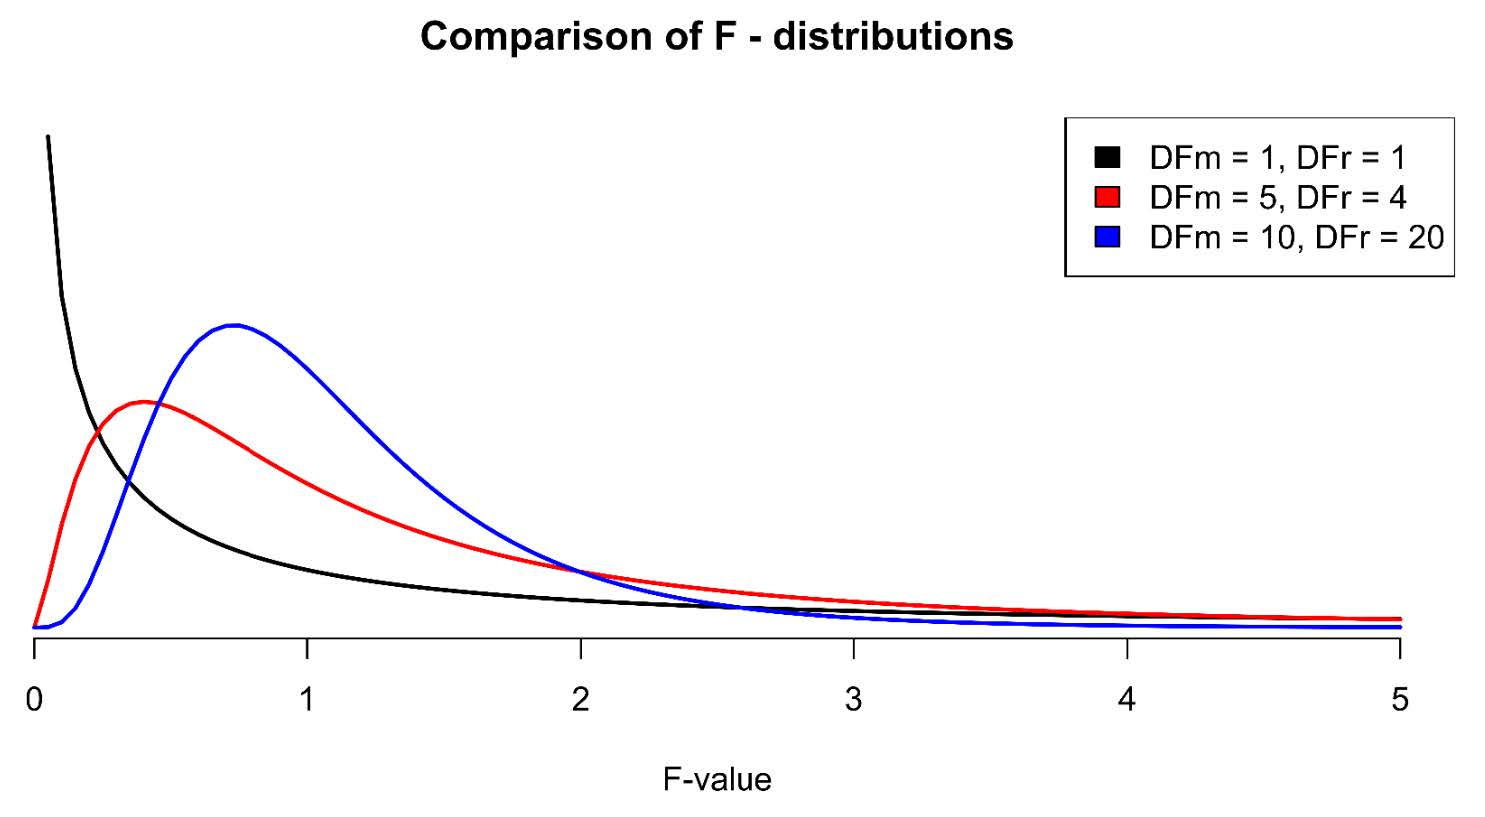
\includegraphics[width=.9\textwidth]{Files/Images/fdistributions.jpg}
\end{center}

\clearpage % Page break

\question{
    6.2 b
}{
    Calculate the \concept{degrees of freedom} $df_M$ and $df_R$ of the \concept{F-distribution} for the data in \rcode{dataset8}.
}

\hint{Hint 6.2: You can find the formulas for $df_M$ and $df_R$ in the formula sheet.}

\emptyanswerbox{
    6.2b
}{
    $df_M$: \shortanswerline \hspace*{3cm} $df_R$: \shortanswerline
}

\question{
    6.2 c
}{
    Using the \rcode{qf()} function, calculate the \concept{critical F-value} that is required to reject the \concept{null hypothesis} $H_0$ for these data with 95\% confidence.
}

\rcodeanswertiny{6.2c}

\emptyanswerbox{
    6.2c
}{
    Critical F-value: \shortanswerline
}

The \rcode{aov()} function in \texttt{R} is a wrapper for the \rcode{lm()} function. The difference between these two functions is that the \rcode{lm()} function can only handle \concept{categorical} predictors with two levels (e.g., a \concept{dummy variable}). The \rcode{aov()} function can handle \concept{categorical} predictor variables with more than two levels, since it automatically rewrites the \rcode{formula} to include the \concept{dummy variables}. \\ 

\question{
    6.2 d
}{
    Use the \rcode{aov()} function to perform an \concept{ANOVA} with the dependent (outcome) variable \rcode{Score} and the independent (predictor) variable \rcode{Group} and store the result in an object named \rcode{anovaResult}.
}

\hint{Hint 6.3: You can check more information on the \rcode{aov()} function with \rcode{?aov}.}

\rcodeanswersmall{6.2d}

\clearpage % Page break

\question{
    6.2 e
}{
    Use the \rcode{summary()} function to inspect the results of the \concept{ANOVA} in \rcode{anovaResult}. What is the \concept{F-value} that is calculated from the \concept{sample}? What is the \concept{p-value} calculated from the \concept{sample}?
}

\rcodeanswertiny{6.2e}

\emptyanswerbox{
    6.2e
}{
    F-value: \shortanswerline \hspace*{3cm} p-value: \shortanswerline
}

\question{
    6.2 f
}{
    What is your conclusion on the basis of these results? Include the following elements:
        \begin{itemize}
        \item[$\square$] Discuss what the \concept{p-value} is for this test.
    \item[$\square$] Discuss whether $H_0$ is rejected or not.
    \item[$\square$] Describe what this tells us about $\mu_{Blue}$, $\mu_{Brown}$, $\mu_{Green}$, and $\mu_{Down}$.  
    \item[$\square$] Describe what type of error is relevant \textit{(type-I or type-II)}.
\end{itemize}
}

\sixlineanswerbox{6.2f}

\clearpage % Page break